\documentclass[dvipsnames, tikz]{standalone}
\usepackage{amsmath}
\usepackage{arevmath}
\usepackage{xcolor}
\usepackage{tikz}
\usetikzlibrary{calc}
\usetikzlibrary{decorations.pathreplacing,calligraphy,3d}
\usetikzlibrary{matrix,shapes,fit,backgrounds}

\def\kleur{black}

\begin{document}
	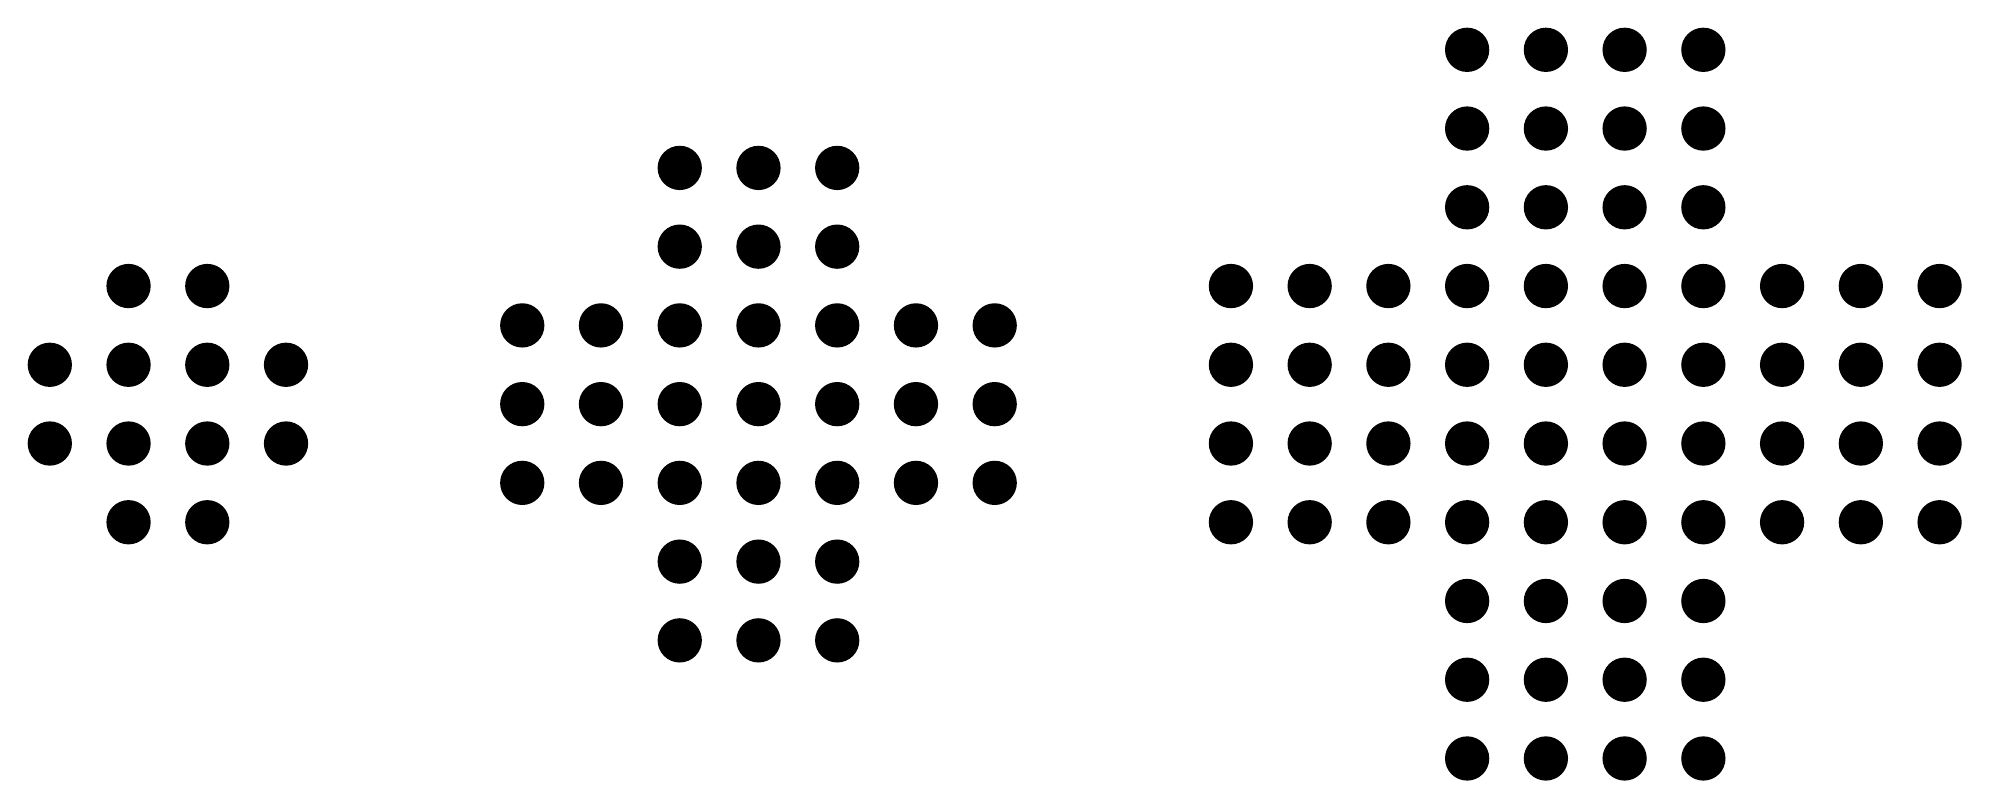
\begin{tikzpicture}
		\foreach \x in {1,...,3}{
			\foreach \y in {1,...,7}{
				\fill[\kleur] (\x, \y) circle (8pt);
			}
		}
		\foreach \x in {1,...,2}{
			\foreach \y in {1,...,3}{
				\fill[\kleur] (-\x+1, \y+2) circle (8pt);
				\fill[\kleur] (\x+3, \y+2) circle (8pt);
			}
		}
	
		\begin{scope}[xshift=10cm, yshift=-1.5cm]
			\foreach \x in {1,...,4}{
				\foreach \y in {1,...,10}{
					\fill[\kleur] (\x, \y) circle (8pt);
				}
			}
			\foreach \x in {1,...,3}{
				\foreach \y in {1,...,4}{
					\fill[\kleur] (-\x+1, \y+3) circle (8pt);
					\fill[\kleur] (\x+4, \y+3) circle (8pt);
				}
			}
		\end{scope}
	
		\begin{scope}[xshift=-7cm, yshift=1.5cm]
			\foreach \x in {1,...,2}{
				\foreach \y in {1,...,4}{
					\fill[\kleur] (\x, \y) circle (8pt);
				}
			}
			\foreach \x in {1,...,1}{
				\foreach \y in {1,...,2}{
					\fill[\kleur] (-\x+1, \y+1) circle (8pt);
					\fill[\kleur] (\x+2, \y+1) circle (8pt);
				}
			}
		\end{scope}
	\end{tikzpicture}
\end{document}